% ============================================================
\chapter{Graph Neural Networks}
\label{ch:gnn}
% ============================================================

Convolutional neural networks revolutionised computer vision, but they rest on an implicit assumption: data lives on a regular grid. What happens when the data is a social network, a molecule, a 3D mesh, or a transportation network? These structures are naturally represented by \emph{graphs}, where the notion of neighbourhood is irregular and variable. The idea of \emph{Graph Neural Networks} (GNNs), formalised by Franco Scarselli in 2009 and then rediscovered and extended by Thomas Kipf, Petar Veli\v{c}kovi\'c, and many others from 2016 onward, is to adapt the convolution mechanism to this irregular geometry: each node updates its representation by aggregating messages from its neighbours.

This \emph{message passing} paradigm has become the unifying framework for learning on graphs. This chapter builds its foundations.

\section{Graph Representation}

\begin{definition}[Attributed graph]
An \textbf{attributed graph} is a tuple $G = (V, E, \mathbf{X}, \mathbf{E})$ where:
\begin{itemize}
    \item $V = \{1, \ldots, n\}$ is the set of \textbf{nodes}.
    \item $E \subseteq V \times V$ is the set of \textbf{edges}.
    \item $\mathbf{X} \in \R^{n \times d}$ is the \textbf{node feature matrix}.
    \item $\mathbf{E} \in \R^{\abs{E} \times d_e}$ contains the \textbf{edge features}.
\end{itemize}
\end{definition}

\begin{definition}[Associated matrices]
For a graph $G = (V, E)$:
\begin{itemize}
    \item \textbf{Adjacency matrix}: $A_{ij} = 1$ if $(i,j) \in E$, $0$ otherwise.
    \item \textbf{Degree matrix}: $D_{ii} = \sum_j A_{ij}$ (diagonal).
    \item \textbf{Laplacian}: $\mathbf{L} = \mathbf{D} - \mathbf{A}$.
    \item \textbf{Normalized Laplacian}:
          $\tilde{\mathbf{L}} = \mathbf{I} - \mathbf{D}^{-1/2}\mathbf{A}\mathbf{D}^{-1/2}$.
\end{itemize}
\end{definition}

\begin{codeblock}[title=\textbf{Graph representation in PyTorch Geometric}]
\begin{minted}{python}
import torch
from torch_geometric.data import Data

# Graph with 4 nodes and 5 edges (undirected)
edge_index = torch.tensor([
    [0, 1, 1, 2, 2, 3, 3, 0, 1, 3],
    [1, 0, 2, 1, 3, 2, 0, 3, 3, 1]
], dtype=torch.long)

# Node features (4 nodes, 3 features)
x = torch.tensor([
    [1.0, 0.0, 0.0],  # node 0: carbon
    [0.0, 1.0, 0.0],  # node 1: nitrogen
    [0.0, 0.0, 1.0],  # node 2: oxygen
    [1.0, 0.0, 0.0],  # node 3: carbon
], dtype=torch.float)

data = Data(x=x, edge_index=edge_index)
print(f"Nodes: {data.num_nodes}, Edges: {data.num_edges}")
print(f"Features: {data.x.shape}")
print(f"Isolated: {data.has_isolated_nodes()}")
print(f"Self-loops: {data.has_self_loops()}")
\end{minted}
\end{codeblock}

\section{The Message Passing Paradigm}

\subsection{General Formalization}

\begin{definition}[Message Passing Neural Network (MPNN)]
An \textbf{MPNN} (Gilmer et al., 2017) updates node representations through
iterations of the form:
\begin{align}
    \mathbf{m}_v^{(\ell+1)} &= \bigoplus_{u \in \mathcal{N}(v)}
    \psi^{(\ell)}\!\left(\mathbf{h}_v^{(\ell)}, \mathbf{h}_u^{(\ell)},
    \mathbf{e}_{uv}\right) \quad \text{(message aggregation)} \label{eq:mpnn_agg} \\
    \mathbf{h}_v^{(\ell+1)} &= \phi^{(\ell)}\!\left(\mathbf{h}_v^{(\ell)},
    \mathbf{m}_v^{(\ell+1)}\right) \quad \text{(update)} \label{eq:mpnn_upd}
\end{align}
where:
\begin{itemize}
    \item $\psi^{(\ell)}$ is the \textbf{message function}.
    \item $\bigoplus$ is a permutation-invariant \textbf{aggregation} operator
          (sum, mean, max).
    \item $\phi^{(\ell)}$ is the \textbf{update function}.
    \item $\mathbf{h}_v^{(0)} = \mathbf{x}_v$ (initial features).
\end{itemize}
\end{definition}

\begin{theorem}[Equivariance of MPNNs]
Any MPNN layer with permutation-invariant aggregation is
\textbf{permutation equivariant}: if $\pi \in S_n$ is a permutation, then:
\[
    \mathbf{h}_{\pi(v)}^{(\ell+1)}(\pi \cdot G) = \mathbf{h}_v^{(\ell+1)}(G)
\]
where $\pi \cdot G$ is the graph with nodes renumbered by $\pi$.
\end{theorem}

\begin{proof}
The aggregation $\bigoplus$ is permutation invariant by assumption. The
functions $\psi$ and $\phi$ are applied individually to each node. The
neighborhood $\mathcal{N}(\pi(v))$ in $\pi \cdot G$ is exactly
$\{\pi(u) : u \in \mathcal{N}(v)\}$ in $G$. Therefore:
\begin{align*}
    \mathbf{m}_{\pi(v)}^{(\ell+1)}(\pi \cdot G)
    &= \bigoplus_{w \in \mathcal{N}(\pi(v))} \psi(\mathbf{h}_{\pi(v)}, \mathbf{h}_w, \mathbf{e}_{w,\pi(v)}) \\
    &= \bigoplus_{u \in \mathcal{N}(v)} \psi(\mathbf{h}_v, \mathbf{h}_u, \mathbf{e}_{uv})
    = \mathbf{m}_v^{(\ell+1)}(G). \qedhere
\end{align*}
\end{proof}

\subsection{Message Passing Illustration}

\begin{figure}[htbp]
\centering
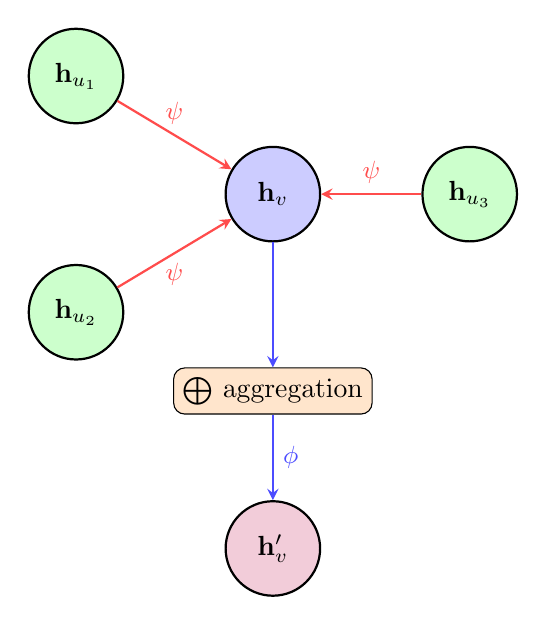
\begin{tikzpicture}[
    node_style/.style={circle, draw, thick, minimum size=12mm, inner sep=0pt},
    msg/.style={->, thick, >=stealth, color=red!70},
    upd/.style={->, thick, >=stealth, color=blue!70}
]
\node[node_style, fill=blue!20] (v) at (0, 0) {$\mathbf{h}_v$};
\node[node_style, fill=green!20] (u1) at (-2.5, 1.5) {$\mathbf{h}_{u_1}$};
\node[node_style, fill=green!20] (u2) at (-2.5, -1.5) {$\mathbf{h}_{u_2}$};
\node[node_style, fill=green!20] (u3) at (2.5, 0) {$\mathbf{h}_{u_3}$};

\draw[msg] (u1) -- node[above, font=\small, color=red!70] {$\psi$} (v);
\draw[msg] (u2) -- node[below, font=\small, color=red!70] {$\psi$} (v);
\draw[msg] (u3) -- node[above, font=\small, color=red!70] {$\psi$} (v);

\node[rectangle, draw, fill=orange!20, rounded corners] (agg) at (0, -2.5)
    {$\bigoplus$ aggregation};
\draw[upd] (v) -- (agg);

\node[node_style, fill=purple!20] (vnew) at (0, -4.5) {$\mathbf{h}_v'$};
\draw[upd] (agg) -- node[right, font=\small, color=blue!70] {$\phi$} (vnew);
\end{tikzpicture}
\caption{Message passing scheme: messages, aggregation, update.}
\end{figure}

\section{Graph Convolutional Network (GCN)}

\begin{definition}[GCN layer --- Kipf and Welling, 2017]
The GCN layer uses the following \textbf{propagation rule}:
\[
    \mathbf{H}^{(\ell+1)} = \sigma\!\left(\hat{\mathbf{D}}^{-1/2}
    \hat{\mathbf{A}}\, \hat{\mathbf{D}}^{-1/2}\, \mathbf{H}^{(\ell)}\,
    \mathbf{W}^{(\ell)}\right)
\]
where:
\begin{itemize}
    \item $\hat{\mathbf{A}} = \mathbf{A} + \mathbf{I}$ (self-loop addition).
    \item $\hat{\mathbf{D}}_{ii} = \sum_j \hat{A}_{ij}$ (adjusted degrees).
    \item $\mathbf{W}^{(\ell)} \in \R^{d_\ell \times d_{\ell+1}}$ is the weight matrix.
    \item $\sigma$ is a nonlinear activation (ReLU).
\end{itemize}
\end{definition}

\begin{remark}[Interpretation]
For a node $v$, the GCN layer computes:
\[
    \mathbf{h}_v^{(\ell+1)} = \sigma\!\left(\sum_{u \in \mathcal{N}(v) \cup \{v\}}
    \frac{1}{\sqrt{\hat{d}_v \hat{d}_u}}\, \mathbf{h}_u^{(\ell)}\, \mathbf{W}^{(\ell)}\right)
\]
This is a \textbf{weighted average} of neighbor representations, followed by
a linear transformation and nonlinearity.
\end{remark}

\begin{proposition}[Connection to the Laplacian]
The GCN layer can be written as:
\[
    \mathbf{H}^{(\ell+1)} = \sigma\!\left((\mathbf{I} - \tilde{\mathbf{L}}_{\text{sym}})
    \mathbf{H}^{(\ell)} \mathbf{W}^{(\ell)}\right)
\]
where $\tilde{\mathbf{L}}_{\text{sym}}$ is the normalized Laplacian of $\hat{G}$
(graph with self-loops). The GCN layer thus performs \textbf{Laplacian smoothing}
of features.
\end{proposition}

\begin{codeblock}[title=\textbf{Complete GCN implementation}]
\begin{minted}{python}
import torch
import torch.nn as nn
import torch.nn.functional as F
from torch_geometric.nn import GCNConv
from torch_geometric.datasets import Planetoid

class GCN(nn.Module):
    def __init__(self, in_channels, hidden_channels, out_channels,
                 num_layers=3, dropout=0.5):
        super().__init__()
        self.convs = nn.ModuleList()
        self.convs.append(GCNConv(in_channels, hidden_channels))
        for _ in range(num_layers - 2):
            self.convs.append(GCNConv(hidden_channels, hidden_channels))
        self.convs.append(GCNConv(hidden_channels, out_channels))
        self.dropout = dropout

    def forward(self, x, edge_index):
        for i, conv in enumerate(self.convs[:-1]):
            x = conv(x, edge_index)
            x = F.relu(x)
            x = F.dropout(x, p=self.dropout, training=self.training)
        x = self.convs[-1](x, edge_index)
        return x

# Node classification on Cora
dataset = Planetoid(root='/tmp/Cora', name='Cora')
data = dataset[0]

model = GCN(dataset.num_features, 64, dataset.num_classes)
optimizer = torch.optim.Adam(model.parameters(), lr=0.01, weight_decay=5e-4)

model.train()
for epoch in range(200):
    optimizer.zero_grad()
    out = model(data.x, data.edge_index)
    loss = F.cross_entropy(out[data.train_mask], data.y[data.train_mask])
    loss.backward()
    optimizer.step()

model.eval()
pred = model(data.x, data.edge_index).argmax(dim=1)
correct = (pred[data.test_mask] == data.y[data.test_mask]).sum()
acc = correct / data.test_mask.sum()
print(f"Test accuracy: {acc:.4f}")
\end{minted}
\end{codeblock}

\section{The Over-Smoothing Problem}

\begin{theorem}[Over-smoothing --- Li et al., 2018]
Stacking $L$ GCN layers causes all node representations to converge to a
fixed point:
\[
    \lim_{L \to \infty} \mathbf{H}^{(L)} = \mathbf{1}\boldsymbol{\pi}^\top \mathbf{H}^{(0)} \mathbf{W}_\infty
\]
where $\boldsymbol{\pi}$ is the dominant eigenvector of the graph (related
to the stationary distribution of the random walk). All nodes obtain the
\textbf{same representation}.
\end{theorem}

\begin{warning}[title=\textbf{Practical consequences}]
\begin{itemize}
    \item Deep GNNs ($L > 5$) often lose performance.
    \item Representations become indistinguishable across nodes.
    \item Solutions: residual connections, normalization, DropEdge.
\end{itemize}
\end{warning}

\section{Readout and Graph-Level Prediction}

\begin{definition}[Readout]
To obtain a graph-level representation from node representations, a
permutation-invariant \textbf{readout} function is used:
\[
    \mathbf{h}_G = \text{READOUT}(\{\mathbf{h}_v^{(L)} : v \in V\})
\]
Common options:
\begin{itemize}
    \item Sum: $\mathbf{h}_G = \sum_{v \in V} \mathbf{h}_v^{(L)}$
    \item Mean: $\mathbf{h}_G = \frac{1}{\abs{V}} \sum_{v \in V} \mathbf{h}_v^{(L)}$
    \item Max: $\mathbf{h}_G = \max_{v \in V} \mathbf{h}_v^{(L)}$
    \item Attention: weighted sum with learned weights.
\end{itemize}
\end{definition}

\section{Expressive Power of GNNs}

\begin{theorem}[Connection to Weisfeiler--Leman test --- Xu et al., 2019]
MPNNs are \textbf{at most as expressive} as the 1-dimensional
Weisfeiler--Leman (1-WL) test. More precisely:
\begin{enumerate}
    \item If 1-WL distinguishes two graphs $G_1$ and $G_2$, then there exists
          an MPNN that distinguishes them.
    \item If 1-WL does not distinguish $G_1$ and $G_2$, then \textbf{no} MPNN
          can distinguish them.
\end{enumerate}
\end{theorem}

\begin{definition}[Weisfeiler--Leman test (1-WL)]
The 1-WL test is an iterative color-refinement algorithm:
\begin{enumerate}
    \item \textbf{Initialization}: $c_v^{(0)} = \text{initial color of } v$.
    \item \textbf{Iteration}: $c_v^{(t+1)} = \text{HASH}\!\left(c_v^{(t)},
          \{\!\!\{c_u^{(t)} : u \in \mathcal{N}(v)\}\!\!\}\right)$
    \item \textbf{Termination}: when colors stabilize.
\end{enumerate}
where $\{\!\!\{\cdot\}\!\!\}$ denotes a multiset.
\end{definition}

\begin{figure}[htbp]
\centering
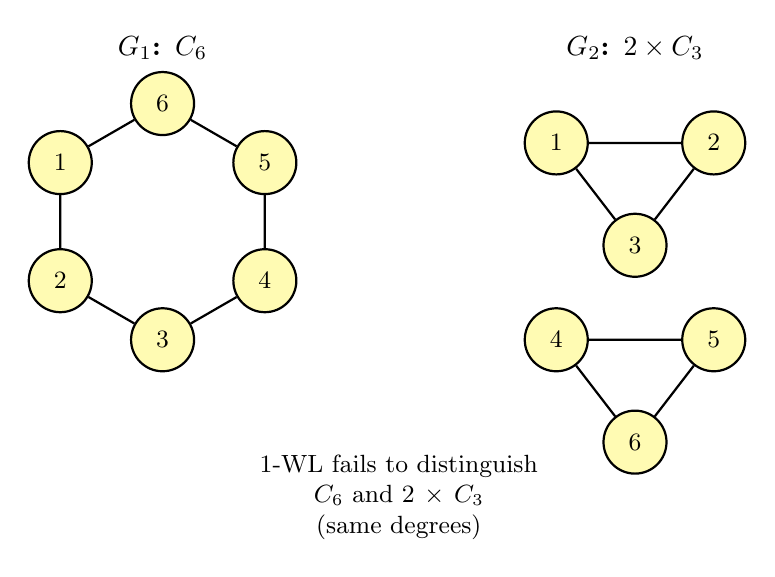
\begin{tikzpicture}[
    node_style/.style={circle, draw, thick, minimum size=8mm, inner sep=0pt, font=\small}
]
% Graph 1: cycle C6
\begin{scope}[shift={(-3,0)}]
    \node[font=\bfseries] at (0, 2.2) {$G_1$: $C_6$};
    \foreach \i in {1,...,6} {
        \pgfmathsetmacro{\angle}{60*\i + 90}
        \node[node_style, fill=yellow!30] (a\i) at (\angle:1.5) {\i};
    }
    \draw[thick] (a1)--(a2)--(a3)--(a4)--(a5)--(a6)--(a1);
\end{scope}
% Graph 2: two triangles
\begin{scope}[shift={(3,0)}]
    \node[font=\bfseries] at (0, 2.2) {$G_2$: $2 \times C_3$};
    \node[node_style, fill=yellow!30] (b1) at (-1, 1) {1};
    \node[node_style, fill=yellow!30] (b2) at (1, 1) {2};
    \node[node_style, fill=yellow!30] (b3) at (0, -0.3) {3};
    \node[node_style, fill=yellow!30] (b4) at (-1, -1.5) {4};
    \node[node_style, fill=yellow!30] (b5) at (1, -1.5) {5};
    \node[node_style, fill=yellow!30] (b6) at (0, -2.8) {6};
    \draw[thick] (b1)--(b2)--(b3)--(b1);
    \draw[thick] (b4)--(b5)--(b6)--(b4);
\end{scope}
\node[font=\small, text width=4cm, align=center] at (0, -3.5)
    {1-WL fails to distinguish\\$C_6$ and $2\times C_3$\\(same degrees)};
\end{tikzpicture}
\caption{Two regular graphs that 1-WL (and thus MPNNs) cannot distinguish.}
\end{figure}

\section{GCN from Scratch}

\begin{codeblock}[title=\textbf{GCN implemented from scratch}]
\begin{minted}{python}
import torch
import torch.nn as nn

class GCNLayerManual(nn.Module):
    """Manually implemented GCN layer."""
    def __init__(self, in_features, out_features):
        super().__init__()
        self.W = nn.Parameter(torch.randn(in_features, out_features) * 0.01)
        self.bias = nn.Parameter(torch.zeros(out_features))

    def forward(self, X, A):
        n = A.size(0)
        A_hat = A + torch.eye(n, device=A.device)
        D_hat = torch.diag(A_hat.sum(dim=1))
        D_inv_sqrt = torch.diag(1.0 / torch.sqrt(A_hat.sum(dim=1)))
        A_norm = D_inv_sqrt @ A_hat @ D_inv_sqrt
        H = A_norm @ X @ self.W + self.bias
        return torch.relu(H)

# Test on a small graph
A = torch.tensor([[0, 1, 0, 1],
                   [1, 0, 1, 0],
                   [0, 1, 0, 1],
                   [1, 0, 1, 0]], dtype=torch.float)
X = torch.randn(4, 8)

layer = GCNLayerManual(8, 16)
out = layer(X, A)
print(f"Output: {out.shape}")  # (4, 16)
\end{minted}
\end{codeblock}

\section{Types of Graph Tasks}

\begin{definition}[Prediction levels]
Graph learning tasks fall into three levels:
\begin{enumerate}
    \item \textbf{Node-level}: node classification, regression
          (e.g., document classification in a citation network).
    \item \textbf{Edge-level}: link prediction, edge classification
          (e.g., recommendation).
    \item \textbf{Graph-level}: classification, regression of entire graphs
          (e.g., molecular property prediction).
\end{enumerate}
\end{definition}

\begin{codeblock}[title=\textbf{Molecular graph classification}]
\begin{minted}{python}
import torch
import torch.nn.functional as F
from torch_geometric.nn import GCNConv, global_add_pool
from torch_geometric.datasets import TUDataset
from torch_geometric.loader import DataLoader

class GraphClassifier(torch.nn.Module):
    def __init__(self, num_features, hidden_dim, num_classes):
        super().__init__()
        self.conv1 = GCNConv(num_features, hidden_dim)
        self.conv2 = GCNConv(hidden_dim, hidden_dim)
        self.conv3 = GCNConv(hidden_dim, hidden_dim)
        self.classifier = torch.nn.Sequential(
            torch.nn.Linear(hidden_dim, hidden_dim),
            torch.nn.ReLU(),
            torch.nn.Dropout(0.5),
            torch.nn.Linear(hidden_dim, num_classes),
        )

    def forward(self, data):
        x, edge_index, batch = data.x, data.edge_index, data.batch
        x = F.relu(self.conv1(x, edge_index))
        x = F.relu(self.conv2(x, edge_index))
        x = F.relu(self.conv3(x, edge_index))
        x = global_add_pool(x, batch)
        return self.classifier(x)

dataset = TUDataset(root='/tmp/PROTEINS', name='PROTEINS')
train_loader = DataLoader(dataset[:900], batch_size=64, shuffle=True)
test_loader = DataLoader(dataset[900:], batch_size=64)

model = GraphClassifier(dataset.num_features, 64, dataset.num_classes)
optimizer = torch.optim.Adam(model.parameters(), lr=0.001)

for epoch in range(100):
    model.train()
    for data in train_loader:
        optimizer.zero_grad()
        out = model(data)
        loss = F.cross_entropy(out, data.y)
        loss.backward()
        optimizer.step()
\end{minted}
\end{codeblock}

\section*{Exercises}

\begin{exercise}[Deriving the GCN layer]
\begin{enumerate}
    \item Start from the spectral convolution $g_\theta * x = U g_\theta(\Lambda) U^\top x$
          and show that the first-order Chebyshev polynomial approximation yields
          the GCN layer.
    \item Explain the role of the renormalization $\hat{\mathbf{A}} = \mathbf{A} + \mathbf{I}$.
\end{enumerate}
\end{exercise}

\begin{exercise}[Receptive field]
Show that after $L$ MPNN layers, the representation of node $v$ depends on all
nodes at distance $\leq L$ in the graph. Deduce the \textbf{receptive field}
of a GNN.
\end{exercise}

\begin{exercise}[Expressivity limitations]
Construct two non-isomorphic graphs on 8 nodes that the 1-WL test cannot
distinguish. Verify experimentally that a GCN produces the same
representations for both graphs.
\end{exercise}

\begin{exercise}[Message passing with edge features]
Extend the from-scratch GCN implementation to support edge features
$\mathbf{e}_{uv} \in \R^{d_e}$ in the message function.
\end{exercise}
